%BEGIN: SIMACT
\section{SIMACT: a 3D Open Source Smart Home Simulator for Activity Recognition with Open Database and Visual Editor}\label{sec:simact}

SIMACT is a smart home infrastructure simulator, developed in Java, designed to help researchers working in the field of activity recognition \cite{bouchard2012simact}. This work is specifically focused on the interaction between an agent and the surrounding environment in the smart house. It is built to reproduce everyday life scenarios, on a step-by-step basis.\\

The simulator was built entirely on Java based technologies. The GUI was based on the swing library, while the 3D renderer was based on the Java Monkey Engine (JMonkey) version 2.0 \cite{jme:online}. For the 3D design, they have used a modelling tool for house design and interior accessories from Google called SketchUp \cite{sketchup:online}.\\

To further detail, we will briefly discuss on the system's architecture, as illustrated in Figure \ref{fig:simact_architecture}.

\begin{figure}[H]
	\centering
	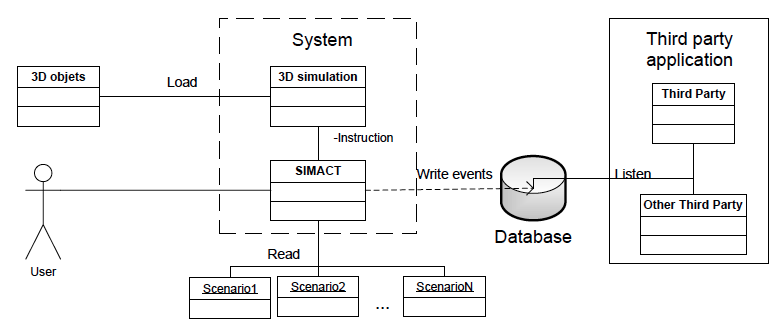
\includegraphics[width=\linewidth]{gfx/Chapter2/simact_architecture}
	\caption{SIMACT: System Architecture}
	\label{fig:simact_architecture}
\end{figure}

To create a custom simulation, a researcher starts out by defining the environment and the object models contained within. The simulator loads these definitions to create the virtual model of the environment and to initialize the 3D simulator. To define the interaction with the habitat, the researcher provides the simulator with an XML file defining the interaction scenario. The scenario is defined as a sequence of steps, which is read, interpreted and execute by the simulator (it plays the role of an interpreter). As the steps are executed and the environment gets modified by these actions, the generated events are written into a database. Further, third party applications can communicate with the database to retrieve data in real-time, which can be used in the logic of the application.\\

A snapshot of the simulation tool in action is depicted in Figure \ref{fig:simact_simulation_tool}.

\begin{figure}[H]
	\centering
	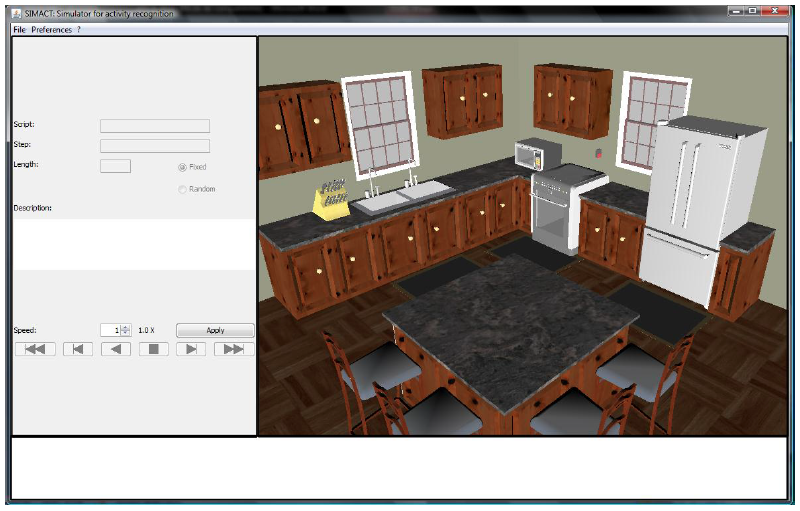
\includegraphics[width=\linewidth]{gfx/Chapter2/simact_simulation_tool}
	\caption{SIMACT: Simulation Tool in Action}
	\label{fig:simact_simulation_tool}
\end{figure}

The novel approach in this simulator is that entire scenarios and interactions can be designed only by using scripts and visual editors, without having to write one line of code. For the 3D design, the researchers have used a modelling tool for house design and interior accessories from Google called SketchUp \cite{sketchup:online}. This comes with a great advantage as SketchUp's community maintains a large library of free 3D models, where one can find almost any accessory that would fit in a home.\\

The framework enables simulation of both devices and physical objects. The entire simulation is controlled by the framework as it interprets the simulation scenario, described in an XML file. This is a step-by-step description of how various parameters of the system (e.g. the temperature in a room) and of objects (e.g. door opened/closed, lamp on/off) evolve. During the simulation, context data can be retrieved by third party service from the data base exposed by the framework.\\

The 3D visualization is a simple animation of the simulation allowing the researcher to look around within the ongoing simulation to better observe the evolution of the system. ''In the 3D zone, one can freely move the camera around the environment to take different points of view and then decide where is the most appropriate position to see what is going on. It is simply done by clicking on the frame and using a keyboard: the arrow keys to rotate and pg up/pg down to zoom'' \cite{bouchard2012simact}.\\

The framework's source code is publicly available as open-source.
%END: SIMACT